% Questo file definisce lo stile che verrà applicato
% ad ogni pagina di contenuto
\documentclass[a4paper,11pt]{article}

\usepackage{ifthen}
\usepackage[
 a4paper,
 top=2.5cm,
 bottom=2.5cm,
 left=1.5cm,
 right=1.5cm,
 head=30pt
]{geometry}
\usepackage[italian]{babel}
\usepackage[utf8x]{inputenc}
\usepackage[T1]{fontenc}
\usepackage{fancyhdr}
\usepackage[colorlinks=true, urlcolor=black, citecolor=black, linkcolor=black]{hyperref}
\usepackage{tabularx}
\usepackage{multirow}
\usepackage{booktabs}
\usepackage{color}
\usepackage[dvipsnames]{xcolor}
\usepackage{graphicx}
\usepackage{eurosym}
\usepackage{amsmath}
\usepackage{relsize}
\usepackage{placeins}
\usepackage{ltablex}
\usepackage{float}

\usepackage[multidot]{grffile}
\usepackage{xcolor,colortbl}
\definecolor{lightblue}{HTML}{56B4E6}
\definecolor{blue}{HTML}{2953A1}
\definecolor{darkblue}{HTML}{1E396E}
\usepackage{longtable}

\usepackage[toc,page]{appendix}
\renewcommand\appendixtocname{Appendice}
\renewcommand{\appendixpagename}{Appendice}

\newcommand\pagenumberingnoreset[1]{\gdef\thepage{\csname @#1\endcsname\c@page}}

% Cambia il font 
\renewcommand*\rmdefault{qhv}

% ***STILE PAGINA***
\pagestyle{fancy}
\fancyhf{}
\setlength{\headheight}{1cm} 
% No indentazione paragrafo
\setlength{\parindent}{0pt}

% ***INTESTAZIONE***
\newcommand\textline[4][t]{%
  \noindent\parbox[#1]{.333\textwidth}{\raisebox{-0.40\height}{#2}}%
  \parbox[#1]{.333\textwidth}{\centering #3}%
  \parbox[#1]{.333\textwidth}{\raggedleft #4}%
}

\lhead{
	\textline[t]{
\includegraphics[width=1cm, keepaspectratio=true]{../../../Template/Logo/Logo.png}}{\progettoShort}{\documento}
}

\renewcommand{\headrulewidth}{0.4pt}  %Linea sotto l'intestazione

% ***PIÈ DI PAGINA***
\lfoot{\textit{\gruppoLink}\\ \footnotesize{\email}}
\rfoot{\thepage} %per le prime pagine: mostra solo il numero romano
\cfoot{}
\renewcommand{\footrulewidth}{0.4pt}   %Linea sopra il piè di pagina


% Ridefinisce command \paragraph{} andando a capo ogni dopo la parola dentro le parentesi ed ha la possibiltà di enumerazione fino a n cifre modificando il numero dentro "secnumdepth"
\usepackage{titlesec}

\setcounter{secnumdepth}{7}
\setcounter{tocdepth}{7}


% Visualizza paragraph come una section
\titleformat{\paragraph}{\normalfont\normalsize\bfseries}{\theparagraph}{1em}{}
\titlespacing*{\paragraph}{0pt}{3.25ex plus 1ex minus .2ex}{1.5ex plus .2ex}

\titleformat{\subparagraph}{\normalfont\normalsize\bfseries}{\thesubparagraph}{1em}{}
\titlespacing*{\subparagraph}{0pt}{3.25ex plus 1ex minus .2ex}{1.5ex plus .2ex}

\makeatletter
\newcounter{subsubparagraph}[subparagraph]
\renewcommand\thesubsubparagraph{%
  \thesubparagraph.\@arabic\c@subsubparagraph}
\newcommand\subsubparagraph{%
  \@startsection{subsubparagraph}    % counter
    {6}                              % level
    {\parindent}                     % indent
    {3.25ex \@plus 1ex \@minus .2ex} % beforeskip
    {0.75em}                           % afterskip
    {\normalfont\normalsize\bfseries}}
\newcommand\l@subsubparagraph{\@dottedtocline{6}{13em}{5.5em}} %gestione dell'indice
\newcommand{\subsubparagraphmark}[1]{}
\makeatother

\makeatletter
\newcounter{subsubsubparagraph}[subsubparagraph]
\renewcommand\thesubsubsubparagraph{%
  \thesubsubparagraph.\@arabic\c@subsubsubparagraph}
\newcommand\subsubsubparagraph{%
  \@startsection{subsubsubparagraph}    % counter
    {7}                              % level
    {\parindent}                     % indent
    {3.25ex \@plus 1ex \@minus .2ex} % beforeskip
    {0.75em}                           % afterskip
    {\normalfont\normalsize\bfseries}}
\newcommand\l@subsubsubparagraph{\@dottedtocline{7}{16em}{6.5em}} %gestione dell'indice
\newcommand{\subsubsubparagraphmark}[1]{}
\makeatother

%Generali
\newcommand{\capitolato}{C5 - Monolith: An interactive bubble provider}
\newcommand{\progettoShort}{Monolith}
\newcommand{\progetto}{Monolith: An interactive bubble provider}
\newcommand{\gruppo}{NPE Developers}
\newcommand{\gruppoLink}{\href{https://gitlab.com/npe-developers}{NpeDevelopers}}
\newcommand{\email}{\href{mailto:npe.developers@gmail.com}{\textcolor{blue}{npe.developers@gmail.com}}}
\newcommand{\password}{NP3Devel0pers}
\newcommand{\myincludegraphics}[2][]{%
	\setbox0=\hbox{\phantom{X}}%
	\vtop{
		\hbox{\phantom{X}}
		\vskip-\ht0
		\hbox{\includegraphics[#1]{#2}}}
}




%Componenti del gruppo
\newcommand{\RM}{Riccardo Montagnin}
\newcommand{\MT}{Manuel Turetta}
\newcommand{\FB}{Francesco Bazzerla}
\newcommand{\SL}{Stefano Lia}
\newcommand{\LD}{Luca Dario}
\newcommand{\DC}{Diego Cavestro}
\newcommand{\ND}{Nicolò Dovico}

%Ruoli
\newcommand{\Pm}{Project Manager}
\newcommand{\Am}{Amministratore}
\newcommand{\AmP}{Amministratori}
\newcommand{\An}{Analista}
\newcommand{\AnP}{Analisti}
\newcommand{\Dev}{Sviluppatore}
\newcommand{\DevP}{Sviluppatori}
\newcommand{\Ver}{Verificatore}
\newcommand{\VerP}{Verificatori}
\newcommand{\Progr}{Programmatore}
\newcommand{\ProgrP}{Programmatori}
\newcommand{\Prog}{Progettista}
\newcommand{\ProgP}{Progettisti}



%Firme
\newcommand{\RMFirma}{\myincludegraphics[scale = 0.5]{../../../Template/Firme/RM.png}}
\newcommand{\MTFirma}{\myincludegraphics[scale = 0.5]{../../../Template/Firme/MT.png}}
\newcommand{\FBFirma}{\myincludegraphics[scale = 0.5]{../../../Template/Firme/FB.png}}
\newcommand{\SLFirma}{\myincludegraphics[scale = 0.5]{../../../Template/Firme/SL.png}}
\newcommand{\LDFirma}{\myincludegraphics[scale = 0.5]{../../../Template/Firme/LD.png}}
\newcommand{\DCFirma}{\myincludegraphics[scale = 0.5]{../../../Template/Firme/DC.png}}
\newcommand{\NDFirma}{\myincludegraphics[scale = 0.5]{../../../Template/Firme/ND.png}}

%Professori e proponente
\newcommand{\TV}{Prof. Tullio Vardanega}
\newcommand{\RC}{Prof. Riccardo Cardin}
\newcommand{\RB}{Red Babel}
\newcommand{\proponente}{Red Babel}

%Documenti
\newcommand{\Gl}{Glossario}
\newcommand{\glossario}{\textit{\Gl\_v.2.0.0.pdf}}
\newcommand{\AdR}{Analisi dei Requisiti}
\newcommand{\analisiDeiRequisiti}{\textit{\AdR\_v.2.0.0.pdf}}
\newcommand{\AdRvDue}{AnalisiDeiRequisiti}
\newcommand{\NdP}{Norme di Progetto}
\newcommand{\normeDiProgetto}{\textit{\NdP\_v.2.0.0.pdf}}
\newcommand{\PdP}{Piano di Progetto}
\newcommand{\pianoDiProgetto}{\textit{\PdP\_v.2.0.0.pdf}}
\newcommand{\SdF}{Studio di Fattibilità}
\newcommand{\studioDiFattibilita}{\textit{\SdF\_v.2.0.0.pdf}}
\newcommand{\PdQ}{Piano di Qualifica}
\newcommand{\pianoDiQualifica}{\textit{\PdQ\_v.2.0.0.pdf}}
\newcommand{\VI}{Verbale Interno}
\newcommand{\VE}{Verbale Esterno}
\newcommand{\ST}{Specifica Tecnica}
\newcommand{\MU}{Manuale Utente}
\newcommand{\DDP}{Definizione di Prodotto}

%Periodo di progetto
\newcommand{\ARM}{Analisi dei Requisiti di Massima}
\newcommand{\ARD}{Analisi dei Requisiti in Dettaglio}
\newcommand{\PA}{Progettazione Architetturale}
\newcommand{\PD}{Progettazione di Dettaglio}
\newcommand{\COD}{Codifica}
\newcommand{\VV}{Verifica e Testing Finale}

%Consegne
\newcommand{\RR}{Revisione dei Requisiti}
\newcommand{\RP}{Revisione di Progettazione}
\newcommand{\RQ}{Revisione di Qualifica}
\newcommand{\RA}{Revisione di Accettazione}


%Formattazione
\newcommand{\termine}[1]{\textit{#1}\small{$_G$}}
\newcommand{\link}[1]{\href{#1}{\textcolor{blue}{\texttt{#1}}}} 

% Testi ricorrenti
\newcommand{\scopoProdotto}{L'obiettivo di questo progetto è la realizzazione di un \termine{SDK} che permetta la creazione di bolle interattive, le quali, successivamente, verranno utilizzate all'interno dell'applicazione di messaggistica istantanea open source \termine{Rocket.chat}. \\
Dopo la realizzazione di tale \termine{SDK}, è proposto lo sviluppo di un'applicazione in grado di sfruttare l'\termine{SDK} per implementare un uso originale. L'applicazione scelta dal \termine{team} consiste nella bolla lista-spesa e nei suoi vari utilizzi all'interno della piattaforma \termine{Rocket.chat}.
}
\newcommand{\descrizioneGlossario}{Al fine di mantenere questo documento compatto e di facile lettura è stato realizzato un glossario esterno contenente tutte le definizioni dei termini che più comunemente verranno presentati al lettore.  
Tale glossario si ritrova all'interno del file \glossario, e contiene tutti e soli i termini che vengono marcati con una \textit{G} a pedice.
}
\newcommand{\riferimentiNormativi}{
	\begin{itemize}
		\item \textbf{Norme di Progetto}: \normeDiProgetto
		\item \textbf{\termine{Capitolato} d'appalto C5: Monolith - An Interactive bubble provider} \\
			  \link{http://www.math.unipd.it/~tullio/IS-1/2016/Progetto/C5.pdf}
	\end{itemize}
}

% Comandi per generare l'intro
\newcommand{\documento}{Monolith's user manual}
\newcommand{\versione}{2.0.0}
\newcommand{\redatori}{\RM\\ & \DC\\}
\newcommand{\revisori}{\LD}
\newcommand{\dataApprovazione}{15th june 2017}
\newcommand{\approvazione}{\FB}
\newcommand{\statoapprovazione}{Approved}
\newcommand{\uso}{External}
\newcommand{\destinatari}{\RB\\ & \TV\\ & \RC}

\newcommand{\sommario}{This documents contains all the information that will be useful to a developer that wants to use \progetto\ while developing his Meteor-based application.}
\usepackage{graphicx}
\usepackage{placeins}
\usepackage{ltablex}
\usepackage{float}
\usepackage{verbatim}


%Questo file si occupa di generare la tabella delle modifiche
\pagenumbering{Roman}

\begin{center}
    \Large{\textbf{Change log}}
    	\\\vspace{0.5cm}
    	\normalsize
    \begin{tabularx}{\textwidth}{cXXcc}
        \textbf{Version} & \textbf{Changes - Motivation} & \textbf{Author} & \textbf{Role} & \textbf{Date} \\\toprule
        \modifiche
    \end{tabularx}
\end{center}

\newpage




\begin{document}
% Questo file contiene il layout della prima pagina
\pagenumbering{gobble}

\title{
\includegraphics[width=8cm, keepaspectratio=true]{../../../Template/Logo/Logo.png} \\
	\documento \\
	Version \versione
}
\date{\dataApprovazione}

\maketitle

\begin{center}

\begin{tabular}{ r | l }
  \textbf{Role} & \textbf{Component} \\
  Redaction & \redatori \\
  Revision & \revisori \\
  Approval & \approvazione \\
  \\
  Condition & \statoapprovazione \\
  Usage & \uso \\
  Recipients & \destinatari
\end{tabular}
\end{center}

\begin{center}
\textbf{Summary\\}
\sommario \\
\vspace{1.5cm}\email
\end{center}

\clearpage

\pagenumbering{arabic}
%Questo file si occupa di generare la tabella delle modifiche
\pagenumbering{arabic}

\begin{center}
    \Large{\textbf{Change log}}
    	\\\vspace{0.5cm}
    	\normalsize
    \begin{tabularx}{\textwidth}{cXXcc}
        \textbf{Version} & \textbf{Changes} & \textbf{Author} & \textbf{Role} & \textbf{Date} \\\toprule
        \modifiche
    \end{tabularx}
\end{center}

\newpage



\renewcommand{\contentsname}{Table of contents}
\tableofcontents

\newpage

% \renewcommand{\listoffigures}{List of figures}
%\listoffigures
% \newpage

\pagenumbering{arabic}

% Questo file contiene il layout della prima pagina
\pagenumbering{gobble}

\title{
\includegraphics[width=8cm, keepaspectratio=true]{../../../Template/Logo/Logo.png} \\
	\documento \\
	Version \versione
}
\date{\dataApprovazione}

\maketitle

\begin{center}

\begin{tabular}{ r | l }
  \textbf{Role} & \textbf{Component} \\
  Redaction & \redatori \\
  Revision & \revisori \\
  Approval & \approvazione \\
  \\
  Condition & \statoapprovazione \\
  Usage & \uso \\
  Recipients & \destinatari
\end{tabular}
\end{center}

\begin{center}
\textbf{Summary\\}
\sommario \\
\vspace{1.5cm}\email
\end{center}

\clearpage

\pagenumbering{arabic}
\section{Usage}
The following section will provide common-case code snapshots to help you perform the most common operations that can be done using Monolith.

\subsection{Widgets}
\subsubsection{TextWidget}
\begin{lstlisting}[language=JavaScript]
// Create a TextWidget
let textWidget = new Monolith.Widget.TextWidget;

// Hide the widget
textWidget.setVisibility(false); // Default is true, which will show is

// Set the text. Markdown notation is also supported
textWidget.setText("Foo");
textWidget.setText("Markdown __is supported__ **too**");

// Set the text color using HEX notation (http://www.color-hex.com/)
textWidget.setTextColor("#C61A10");

// Set the text size in pixel
textWidget.setTextSize(15);

// Set the URL highlighting color
textWidget.setUrlHighligthColor("#EE42F4");

// Enable or disable the text formatting, this includes also URL highlighting
textWidget.setFormatText(true);
textWidget.setFormatText(false);
\end{lstlisting}
~\\~\\

\subsubsection{ImageWidget}
\begin{lstlisting}[language=JavaScript]
// Create the ImageWidget
let imageWidget = new Monolith.Widget.ImageWidget;

// Hide the widget
imageWidget.setVisibility(false); // Default is true, which will show is

// Set the image associated with the widget
imageWidget.setImage("path/to/image.png");

// Set the image dimensions
imageWidget.setWidth(200);
imageWidget.setHeight(50);
\end{lstlisting}

\newpage
\subsubsection{ButtonWidget}
\begin{lstlisting}[language=JavaScript]
// Create a ButtonWidget
let buttonWidget = new Monolith.Widget.ButtonWidget;

// Set the dimensions of the button
buttonWidget.setWidth(100);
buttonWidget.setHeight(50);

// Set the color of the button
buttonWidget.setBackgroundColor("#41F492");

// Set the action associated with the button
buttonWidget.setOnClickAction(function(){
    alert("The button has been clicked");
});

// Set the action associated with the button when the user long-clicks it
buttonWidget.setOnLongClickAction(function(){
    alert("The button has been long clicked");
});

// Set the milliseconds that need to pass before a click is considered a long click
buttonWidget.setOnLongClickActionTimer(500);
\end{lstlisting}
~\\~\\

\subsubsection{ListWidget}
\begin{lstlisting}[language=JavaScript]
// Create the ListWidget
let listWidget = new Monolith.Widget.ListWidget;

// Add items to the list
listWidget.addItem("First");
listWidget.addItem("Second");
listWidget.addItem("Third");

// Set the indicator of the list
listWidget.setCharacterNumber(); // Numbered list
listWidget.setCharacterCircle(); // Unnumbered list

// Set the indicator color
listWidget. setColor("#292929");
\end{lstlisting}

\newpage
\subsubsection{CheckListItemWidget}
\begin{lstlisting}[language=JavaScript]
// Create a new CheckListItemWidget
let checkListItemWidget = new Monolith.Widget.CheckListItemWidget;

// Set the text associated with the item
checkListItemWidget.setText("Click me!");

// Customize the check appereance
// Color the check box instead of using a check tick
checkListItemWidget.setUseSelectionMark(true); 
// Set the color that will be used to color the check box
checkListItemWidget.setSelectionColor("#AAAAAA"); 
// Use a check tick
checkListItemWidget.setUseSelectionMark(false); 
// Set the character used as check tick
checkListItemWidget.setSelectionCharacter("X"); 

// Check or un-check the option
checkListItemWidget.setChecked(true); // Checked
checkListItemWidget.setChecked(false); // Un-checked

// Know it the option is checked or not
let isChecked = checkListItemWidget.isChecked();
if (isChecked){
    // The option is checked
} else {
    // The option is not checked
}


// Set the action to perform on click
checkListItemWidget.setOnClick(function(item){
    // The item parameter represents the view of the item that has been clicked
    item.setText("New text after click");
});

// Set the action to perform after a long click (1000 ms)
checkListItemWidget.setOnLongClick(function(){
    // The item parameter represents the view of the item that has been clicked
   item.setText("New text after long click");
});


// Delete the item
checkListItemWidget.removeOption();
\end{lstlisting}

\newpage
\subsubsection{Create a custom widget}
In order to create a new custom widget and add it to \termine{Monolith} so than you can use it like the default ones, you have to do as follows.
\begin{enumerate}

	\item Create a new class which extends from \texttt{BaseWidget}
\begin{lstlisting}[language=JavaScript]
export class MyWidget extends Monolith.Widget.BaseWidget {

    constructor(){
        super(); // You need to call this to create the above hierarchy
        
        // Initialize your widget here
    }
    
    renderView(){
        // Renders the view of the widget and returns a DOMElement object
    }

    performOperation(){
        // Perform some operation
    }

}
\end{lstlisting}

	\item Use your widget wherever you want
\begin{lstlisting}[language=JavaScript]
// Import the widget
import {MyWidget} from '/path/to/MyWidget.js';

// Istantiate the widget
let myWidget = new MyWidget();

// Perform operations with the widget
myWidget.performOperation();

// Render the widget's view
myWidget.renderView();
\end{lstlisting}
  
\end{enumerate}  
  
\textbf{Note} \\ 
The default widget's behaviour does \textbf{not} let the user use a single widget without a bubble container that holds it. \\
If you plan to render the widget's view inside a Rocket.chat room, please create a bubble and add your widget to the bubble, so that the bubble will render it and show it to the user.

\newpage


\subsubsection{Layouts}
Inside \progettoShort\ there are two classes which gives the possibility of arranging the different widgets in two main orientations:
\begin{itemize}
	\item \texttt{HorizontaLayout}: it allows the widgets that are added to it to be displayed each one on the right of the previous ones;
	\item \texttt{VerticalLayout}: it allows the widgets to be displayed one below the previous ones.
\end{itemize}

\paragraph{Using a layout}
To use one of the given layout classes, all that needs to be done is the following:

% Immagine layout prima dell'aggiunta di un widget
\begin{lstlisting}[language=JavaScript, frame=single]
// Needed to be able to create the new layout
import {HorizontalLayout} from {BOH}

let widget = new TextWidget();

let layout = new HorizontalLayout();
layout.addComponent(widget);
\end{lstlisting}
% Immagine layout dopo l'aggiunta del widget

\paragraph{Creating a new layout}
In order to create a new layout class, the only thing that needs to be done is creating a new class which extends from \texttt{BaseLayout} and implements its abstract methods:
\begin{lstlisting}[language=JavaScript, frame=single]
// Needed to be able to create the new layout
import {BaseLayout} from {BOH}

export class MyLayout extends BaseLayout {
    constructor(){
        // Needed in order to create the base class instance
        super();
    }
    
    renderView(){
        // Renders the layout view usually calling its components' 
        // renderView() method and returns the HTML code
    }

}
\end{lstlisting}
\subsubsection{BaseBubble}

\label{BaseBubble}
\begin{figure}[ht]
	\centering
	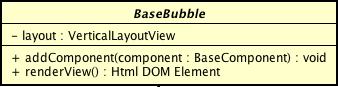
\includegraphics[scale=0.5]{Sezioni/SottosezioniST/img/BaseBubble.png}
	\caption{BaseBubble}
\end{figure}

\begin{itemize}
\item \textbf{Descrizione:} Classe base astratta che rappresenta le bolle di Monolith.
\item \textbf{Utilizzo:} Classe base astratta utilizzata ed estesa ogni qualvolta uno sviluppatore intende creare nuove bolle.
\item \textbf{Attributi:} 
\begin{itemize}
\item \textit{protected layout:VerticalLayoutView}\\
Oggetto che rappresenta il layout verticale della bolla.
\end{itemize}
\item \textbf{Metodi:}
\begin{itemize}
\item \textit{public addComponent(component:BaseComponent):void}\\
Aggiunge un widget alla bolla.
\item{\textbf{Parametri}: \begin{itemize}
\item \textit{component:BaseComponent}\\
Oggetto che rappresenta il componente che si desidera aggiungere alla bolla.
\end{itemize}}
\item \textit{public renderView():string}\\
Genera il codice HTML, CSS e JavaScript necessario per visualizzare bolle.
\end{itemize}
\end{itemize}

\subsubsection{ToDoListBubble}

\label{ToDoListBubble}
\begin{figure}[ht]
	\centering
	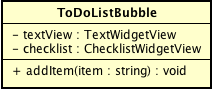
\includegraphics[scale=0.5]{Sezioni/SottosezioniST/img/ToDoListBubble.png}
	\caption{ToDoListBubble}
\end{figure}

\begin{itemize}
\item \textbf{Descrizione:} Classe concreta che estende BaseBubble, destinata alla creazione di bolle lista di Monolith.
\item \textbf{Utilizzo:} Classe utilizzata ogni qualvolta uno sviluppatore intende creare nuove bolle lista.
\item \textbf{Attributi:}
\begin{itemize}
\item \textit{private textView:TextWidgetView}\\
Oggetto che rappresenta il widget contenente il testo della bolla lista.
\item \textit{private checklist:CheckListView}\\
Oggetto che rappresenta il widget contenente la lista di oggetti che si possono spuntare.
\end{itemize}
\item \textbf{Metodi:}
\begin{itemize}
\item \textit{public ToDoListBubble():ToDoListBubble}\\
Il costruttore della classe ToDoListBubble.
\item \textit{public addItem(item:string):void}\\
Aggiunge un elemento con il nome definito alla bolla lista.
\item{\textbf{Parametri}: \begin{itemize}
\item \textit{item:string}\\
Valore che rappresenta il nome dell'elemento che si vuole aggiungere alla lista.
\end{itemize}}
\end{itemize}
\end{itemize}

\subsubsection{MarkdownBubble}

\label{MarkdownBubble}
\begin{figure}[ht]
	\centering
	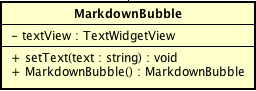
\includegraphics[scale=0.5]{Sezioni/SottosezioniST/img/MarkdownBubble.png}
	\caption{MarkDownBubble}
\end{figure}

\begin{itemize}
\item \textbf{Descrizione:} Classe concreta che estende BaseBubble, destinata alla creazione di bolle testo markdown di Monolith.
\item \textbf{Utilizzo:} Classe utilizzata ogni qualvolta uno sviluppatore intende creare nuove bolle testo markdown.
\item \textbf{Attributi:}
\begin{itemize}
\item \textit{private textview:TextWidgetView}\\
Oggetto che rappresenta il widget contenente il testo della bolla testo markdown.
\end{itemize}
\item \textbf{Metodi:}
\begin{itemize}
\item \textit{public MarkdownBubble():MarkdownBubble}\\
Il costruttore della classe MarkdownBubble.
\item \textit{public setText(text:string):void}\\
Imposta il testo della bolla lista con il valore definito.
\item{\textbf{Parametri}: \begin{itemize}
\item \textit{text:string}\\
Valore che rappresenta il testo che si vuole inserire nella bolla testo markdown.
\end{itemize}}
\end{itemize}
\end{itemize}

\subsubsection{AlertBubble}

\label{AlertBubble}
\begin{figure}[ht]
	\centering
	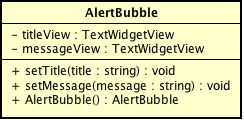
\includegraphics[scale=0.5]{Sezioni/SottosezioniST/img/AlertBubble.png}
	\caption{AlertBubble}
\end{figure}

\begin{itemize}
\item \textbf{Descrizione:} Classe concreta che estende BaseBubble, destinata alla creazione di bolle avviso di Monolith.
\item \textbf{Utilizzo:} Classe utilizzata ogni qualvolta uno sviluppatore intende creare nuove bolle avviso.
\item \textbf{Attributi:} 
\begin{itemize}
\item \textit{private titleView:TextWidgetView}\\
Campo che rappresenta e contiene il titolo della bolla avviso.
\item \textit{private messageView:TextWidgetView}\\
Campo che rappresenta e contiene il messaggio della bolla avviso.
\end{itemize}
\item \textbf{Metodi:}
\begin{itemize}
\item \textit{public AlertBubble():AlertBubble}\\
Il costruttore della classe AlertBubble.
\item \textit{public setTitle(title:string):void}\\
Imposta il titolo della bolla avviso con il valore title.
\item{\textbf{Parametri}: \begin{itemize}
\item \textit{title:string}\\
Valore che rappresenta il titolo che si vuole impostare alla bolla avviso.
\end{itemize}}
\item \textit{public setMessage(message:string):void}\\
Imposta il messaggio della bolla avviso con il valore message.
\item{\textbf{Parametri}: \begin{itemize}
\item \textit{message:string}\\
Valore che rappresenta il messaggio testuale che si vuole impostare alla bolla avviso.
\end{itemize}}
\end{itemize}
\end{itemize}

\newpage
\section{Tests}
Our project comes with several tests already written and ready to execute. \\
We used these tests during the development of the \termine{SDK} in order to be sure that the increments that were performed didn't break the code previously written. \\
We highly suggest you to keep running those tests sometimes, in order to be sure that, if you modify the source code for the application, anything breaks and stop functioning properly. \\


\subsection{Libraries and frameworks}
In order to write and execute the tests, we used the following libraries and frameworks:
\begin{itemize}
	\item \url{Mocha}{https://mochajs.org/}: framework used to execute the test;
	\item \url{Should.js}{https://github.com/shouldjs/should.js}: assertion library;
	\item \url{Expect.js}{https://github.com/LearnBoost/expect.js}: preferred assertion library, as it comes with multiple features that are not present inside Should.js;
	\item \url{Chai.js}{http://chaijs.com/}: another assertion library.
\end{itemize}

\subsection{Running the tests}
In order to run the tests suite, execute the following command inside the folder which contains the \termine{Meteor} project code that includes \termine{Monolith} as a dependency:

\begin{lstlisting}
    meteor test-packages --driver-package practicalmeteor:mocha monolith
\end{lstlisting}

After executing this command, all the unit and integration tests will be run, and the results will be presented at the following url

\begin{lstlisting}
    http://localhost:3000
\end{lstlisting}

where \texttt{localhost} is the server inside which the project using \termine{Monolith} is running.

\newpage
\section{Glossary}
\section*{B}
\addcontentsline{toc}{section}{B}
\begin{itemize}
	\item
	\textbf{Best Practice}: Insieme delle attività che, organizzate in modo sistematico, possono essere prese come riferimento e riprodotte per favorire il raggiungimento dei risultati migliori.
	\item
	\textbf{Bitbucket}: Servizio di hosting per progetti software.
	\item
	\textbf{Bolla}: Ogni messaggio presente all'interno di \termine{Monolith} e, più in generale di \termine{Rocket.chat}, che l'utente può visualizzare all'interno di una qualsiasi chat.
	\item
	\textbf{Bolle Interattive}: Messagio in grado di cambiare il proprio contenuto dopo essere stato inviato.
	\item
	\textbf{Bot}: Programma che accede alla rete attraverso lo stesso tipo di canali utilizzati dagli utenti umani, e che nel nostro caso invia messaggi all'interno di una chat offrendo servizi utili agli utenti.
	\item
	\textbf{Bottone Semplice}: Oggetto che genera eventi alla sua pressione.
	\item
	\textbf{Browser}: E' un'applicazione per il recupero, la presentazione e la navigazione delle risorse sul web.
	\item
	\textbf{Business}: Termine inglese che identifica in generale un'attività economica e approssimativamente può essere tradotto con il termine italiano \textit{affari}.
\end{itemize}
\newpage
\section{G}
\begin{itemize}
	\item
	\textbf{Ganttchart}: \textit{eng. Diagramma di Gantt} Strumento di supporto alla gestione dei progetti usato principalmente nelle attività di project management e costruito partendo da un asse orizzontale -- che rappresenta dell'arco temporale totale del progetto, suddiviso in fasi incrementali (ad esempio, giorni, settimane, mesi) -- e da un asse verticale -- che rappresenta delle mansioni o attività che costituiscono il progetto.
	\item
	\textbf{Gesture}: Gesto a cui è associata una azione.
	\item
	\textbf{Git}: Software di controllo di versione distribuito utilizzabile da interfaccia a riga di comando.
	\item
	\textbf{Github}: Servizio di hosting per progetti software.
	\item
	\textbf{Gitlab}: Servizio di hosting per progetti software.
	\item
	\textbf{Google Drive}: Servizio web di archiviazione di file.
	\item
	\textbf{Grafo Di Controllo Di Flusso}: Grafo che mostra il flusso di esecuzione di un programma, usato per calcolare la \termine{Complessità Ciclomatica}.
	\item
	\textbf{Gruppo}: Insieme delle persone fisiche Diego Cavestro, Francesco Bazzerla, Luca Dario, Manuel Turetta, Nicolò Dovico, Stefano Lia e Riccardo Montagnin.
\end{itemize}
\newpage
\section{J}
\begin{itemize}
	\item
	\textbf{Javascript}: Linguaggio di scripting orientato agli oggetti e agli eventi, comunemente utilizzato nella programmazione Web lato client per la creazione, in siti web e applicazioni web, di effetti dinamici interattivi tramite funzioni di script invocate da eventi innescati a loro volta in vari modi dall'utente sulla pagina web in uso.
	\item
	\textbf{Jenkins}: Strumento open source di continuous integration, scritto in linguaggio Java e che fornisce dei servizi di integrazione continua per lo sviluppo del software.
	\item
	\textbf{Jolie}: Linguaggio di programmazione orientato ai micro servizi.
	\item
	\textbf{Jquery}: Libreria JavaScript per applicazioni web. Nasce con l'obiettivo di semplificare la selezione, la manipolazione, la gestione degli eventi e l'animazione di elementi DOM in pagine HTML, nonché per implementare funzionalità AJAX.
	\item
	\textbf{Jshint}: Strumento di analisi statica del codice volto al linguaggio \termine{JavaScript}.
\end{itemize}
\newpage
\subsection*{R}
\begin{itemize}
	\item
	\textbf{Rocket.Chat}: Rocket.Chat is a Web Chat Server, developed in JavaScript, using the Meteor fullstack framework. It is a great solution for communities and companies wanting to privately host their own chat service or for developers looking forward to build and evolve their own chat platforms..
\end{itemize}
\newpage
\subsection*{S}
\begin{itemize}
	\item
	\textbf{Sdk}: A software development kit (SDK or devkit) is typically a set of software development tools that allows the creation of applications for a certain software package, software framework, hardware platform, computer system, video game console, operating system, or similar development platform..
\end{itemize}
\newpage



\end{document}